\chapter{Hardware jídelní čtečky}

Hardware je založen na mikropočítači, který je osazen procesorem s architekturou ARM.
Z mnoha dnes dostupných ARM počítačů jsem zúžili výběr na následující čtyři:
Omega 2, NanoPi Neo, Orange Pi Zero a VoCore 2.
Tato zařízení byla uvážena, protože jsou malá a mají nainstalovaný ethernet port,
který je nezbytný pro připojení do k ostatním komponentám,
protože jsme nechtěli zvolit bezdrátové připojení do sítě,
které bývá nestabilní a nespolehlivé.

VoCore 2 vyhovoval ve všech bodech, ale byl zamítnut kvůli vysoké ceně.
Omega 2 bylo zamítnuto, protože nebyla žádná výhoda oproti konkurenci.
NanoPi Neo a Orange Pi Zero jsou velmi podobné.
Zprvu bylo zvoleno Orange Pi Zero díky nepatrně lepší výbavě.

\section{Displej a NFC čtečka}

Pro zobrazení pro koncové uživatele byl vybrán standardní rezistivně dotykový displej o
rozlišení 480 na 320 pixelů a o průměru 4 place. Ten komunikuje s počítačem pomocí protokolu SPI,
aby byla dosažena nízká odezva a plynulost displeje. Tento displej je použit pro obsluhu čtečky.
Naopak pro strávníky je zde displej s technologií OLED, rozlišením 128x64 pixelů,
průměrem $1,3$ palce, modré barvy.

Roli samotného čtení čipů nebo mobilů, zajišťuje NFC čtečka založena na
čipu PN532 a desce 3. verze. Modul čte na frekvenci 13,56 MHz.

\section{Napájení}

Napájení Orange Pi Zero (dále už jen OPZ) bylo navrženo s technologií PoE (Power over Ethernet),
kde OPZ má na své desce rospojené spojení pro vypnutí této funkce.
Stačilo tedy jen spojit vývody na desce pomocí cínu.
Tím se krajní piny ethernet portu propojí s interním regulátorem OPZ.
Tím se zjednoduší zapojení, ale pokud spojení přesáhne 10 metrů,
začne se snižovat napětí díky vysokému odporu ethernetového drátu,
což má za následek nedostatečné napájení pro čtečku.

\section{Potíže s SPI a volba Raspberry Pi A+}

Při zapojení jsme zjistili, že OPZ obsahuje jen dva přepínací porty SPI,
což je dostačující pro dotykový displej (obraz a dotyk), ale poté nezbývají
další SPI piny pro OLED displej ani čtečku, které měly být také připojeny pomocí
SPI pro dosažení nízké latence. Proto byla NFC čtečka přepnuta do protokolu I2C,
a tím byla zajištěna komunikace. U displeje byl problém obtížnější, protože 
přepínání protokolů je zajištěno odporem mezi spojeními. Pro obavu z poškození
displeje byl displej vyměněn za jeho menší verzi (0,96 palce), který
nativně podporuje protokol I2C, a tím se vyřešily problémy s počtem pinů.

Počítač byl nakonec nahrazen za Raspberry Pi A+ první generace kvůli softwarové
nekompatibilitě grafiky dotykového displeje. Ten nativně neobsahuje ethernetový port,
a proto musel být použit adaptér z USB na ethernet port, pomocí kterého je zajištěna komunikace
se serverem a opravňování softwaru přes protokol SSH.
Upravování kódu je díky tomu možné pouze přes SSH, protože počítač má jen jeden
USB port a bylo by velmi časově náročné provádět úpravy pomocí dotykového displeje.
Všechny komponenty hardwaru jsou vidět na obrázku~\ref{hardwareGraph}.

\begin{figure} \centering
    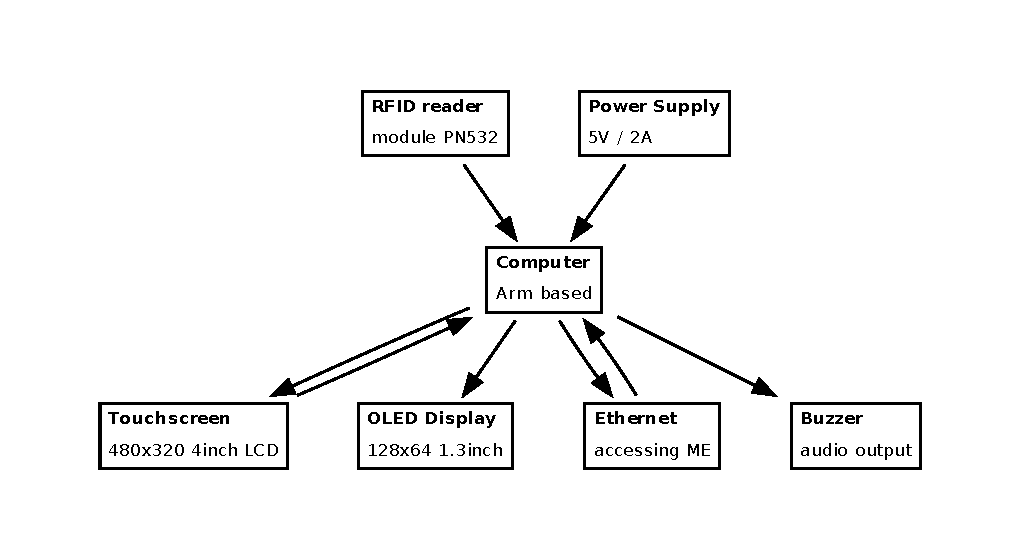
\includegraphics[width=145mm]{../img/hardware}
\caption{Hardware schéma}
\label{hardwareGraph}
\end{figure}

% ORIGNAL TEXT:
% Hardware je založen na mikropočítači, který je osazen procesorem s architekturou typu ARM.
% Z mnoha dnes dostupných ARM počítačů jsem zúžili výběr na následující čtyři:
% Omega 2, NanoPi Neo, Orange Pi Zero a VoCore 2.
% Ty byly vybrány díky své malé velikosti a nainstalovaným ethernet portem,
% který je nezbytný pro připojení do databaze,
% protože jsme nechtěli zvolit připojení do sítě pomocí wifi,
% které je podle našeho názorů nestabilní a nespolehlivé.

% VoCore 2 vyhovoval ve všech bodech, ale byl zamítnut díky vysoké ceně.
% Omega 2 bylo zamítnuto, protože nebyla žádná výhoda oproti konkurenci.
% NanoPi Neo a Orange Pi Zero jsou velmi podobné.
% Nakonec jsme zvolili Orange Pi Zero díky nepatrně lepší výbavě.

% Pro zobrazení pro koncové uživatele jsme vybrali standardní rezistivně dotykový displej o
% rozlišení 480x320 pixelů a průměrem 4 place. Ten komunikuje s počítačem pomocí protokolu SPI,
% aby byla dosažena nízká odezva a plynulost displeje. Tento displej je použit pro obsluhu čtečky.
% Naopak pro strávníky je zde displej s technologií OLED, rozlišením 128x64 pixelů,
% průměrem 1,3 palce, modré barvy. Zde jsou zobrazeny informace určeny pro strávníka.


% Roli samotného čtení čipů nebo mobilů, zajišťuje NFC čtečka založena na
% čipu PN532 a desce 3. verze. Modul čte na frekvenci 13,56 MHz.

% Napájení Orange Pi Zero (Dále už jen OPZ) jsme navrhli pomocí PoE (Power over Ethernet),
% kde OPZ má na své desce rozpojené spojení pro vypnutí této funkce.
% Stačilo tedy jen spojit vývody na desce pomocí cínu.
% Tím se krajní piny ethernet portu propojí s interním regulátorem OPZ.
% Tím se zjednoduší zapojení, ale pokud spojení přesáhne 10 metrů
% začne se snižovat napětí díky vysokému odporu ethernetového drátu,
% což má za následek nedostatečné napájení pro čtečku.

% Při zapojení jsme zjistili, že OPZ obsahuje jen dva přepínací porty SPI,
% což je dostačující pro dotykový displej (obraz a dotyk), ale poté nezbývají
% další SPI piny pro OLED displej ani čtečku, které měly být také připojeny pomocí
% SPI pro dosažení nízké latence. Proto jsme NFC reader přepnuli do protokolu I2C,
% a tím jsme zajistili komunikaci. U displeje byl problém složitější, protože 
% přepínání protokolů je zajištěno odporem mezi spojeními. Pro obavu z poškození
% displeje jsme vyměnili displej za jeho menší verzi (0,96 palce), který má
% nativně podporuje protokol I2C a tím se vyřešily problémy s počtem pinů.

% Počítač byl nahrazen za Raspberry Pi A+ první generace, díky softwarové
% nekompatibilitě grafiky dotykového displeje. Ten nativně neobsahuje ethernetový port,
% a proto byl dodán adaptér z usb na ethernet port, pomocí kterého je zajištěna komunikace
% se serverem a opravnování softwaru přes protokol SSH.
% Upravování kódu je díky tomu možné pouze přes SSH, protože počítač má jen jedno
% usb a bylo by velmi časově náročné provádět úpravy pomocí dotykového displeje.